\documentclass{article}

% Language and Font Settings
\usepackage{fontspec} % Use fontspec to load system fonts in XeTeX
\usepackage{alphabeta}
\usepackage{cite} % Greek letters to Latin encoding for XeTeX

% Set main text font (GFS Didot for Greek)
\setmainfont{Arial} % Sets the main font to GFS Didot for Greek

% Set sans-serif font for section titles
\newfontfamily\greeksf{Franklin Gothic Medium}
\newfontfamily\greekduth{Franklin Gothic Medium}
\newfontfamily\greektitle{Franklin Gothic Book}
\newfontfamily\tabulars{Times New Roman}
\newfontfamily\coding{Consolas}
\newfontfamily\cambria{Cambria}

% Section Font Settings
\usepackage{titlesec}
\titleformat*{\section}{\Large\greeksf} 
\titleformat*{\subsection}{\large\greeksf} 
\titleformat*{\subsubsection}{\greeksf} 

% Set page size and margins
\usepackage[letterpaper,top=2cm,bottom=2cm,left=3cm,right=3cm,marginparwidth=1.75cm]{geometry}
% Useful packages
\usepackage{amsmath}
\usepackage{graphicx}
\graphicspath{ {./images/} }
\usepackage[colorlinks=true, allcolors=blue]{hyperref}
\usepackage{indentfirst}
\usepackage{array}
\usepackage[table,xcdraw]{xcolor}
\usepackage{caption}
\usepackage{multicol}
\usepackage{float}
\usepackage[table,xcdraw]{xcolor}
\usepackage{url}
\usepackage{tabularx}
\usepackage{makecell}
\usepackage{listings}
\usepackage{wrapfig}
\usepackage[bottom]{footmisc}
\usepackage[letterspace=150]{microtype}

\lstdefinestyle{customc}{
  belowcaptionskip=1\baselineskip,
  breaklines=false,
  language=C,
  showstringspaces=false,
  basicstyle=\small\coding,
  keywordstyle=\bfseries\color{red!40!black},
  commentstyle=\itshape\color{purple!40!black},
  identifierstyle=\color{gray},
  stringstyle=\color{orange},
}

\lstdefinestyle{customasm}{
  belowcaptionskip=1\baselineskip,
  frame=L,
  language=SQL,
  basicstyle=\small\coding,
  commentstyle=\itshape\color{purple!40!black},
}

\lstset{escapechar=@,style=customc}
\renewcommand{\contentsname}{Περιεχόμενα}

\renewcommand{\arraystretch}{2}

\begin{document}

\begin{titlepage}
	\centering
	\greekduth
	
\includegraphics[width=0.15\textwidth]{images/duth}\par\vspace{0.5cm}
	{\large\textsc{ΔΗΜΟΚΡΙΤΕΙΟ ΠΑΝΕΠΙΣΤΗΜΙΟ ΘΡΑΚΗΣ}\par}
	\vspace{0.1cm}
	{\large\textsc{ΠΟΛΥΤΕΧΝΙΚΗ ΣΧΟΛΗ}\par}
	\vspace{0.1cm}
	{\large\textsc{ΤΜΗΜΑ ΗΛΕΚΤΡΟΛΟΓΩΝ ΜΗΧΑΝΙΚΩΝ ΚΑΙ ΜΗΧΑΝΙΚΩΝ ΥΠΟΛΟΓΙΣΤΩΝ}\par}
	\vspace{4cm}
	{\lsstyle\greektitle\large\textsc{ΑΣΦΑΛΕΙΑ ΣΥΣΤΗΜΑΤΩΝ ΥΠΟΛΟΓΙΣΤΩΝ}\par}
	\vspace{0.25cm}
	{\huge\bfseries Υλοποίηση IDS με χρήση του εργαλείου Zeek\par}
	\vspace{0.25cm}
	{\greektitle\large\textsc{ΕΡΓΑΣΙΑ ΕΞΑΜΗΝΟΥ}\par}
	\vspace{2cm}
	{Μπούρας Αντώνιος [ΑΕΜ: 58287]\\
	\texttt{antobour1@ee.duth.gr}\\
	Σιδέρης Πέτρος [ΑΕΜ: 58341]\\
	\texttt{petrside@ee.duth.gr}\\
	Ταχτατζής Αναστάσιος [ΑΕΜ: 58439]\\
	\texttt{anastach2@ee.duth.gr}
	\par}
	\vfill
	Υπεύθυνος καθηγητής:\par
	Αναγνωστόπουλος Μάριος

	\vfill

% Bottom of the page
	{\large 13 Ιανουαρίου, 2025\par}
\end{titlepage}
{
  \hypersetup{linkcolor=black}
  \tableofcontents
}
\newpage

\section{Εισαγωγή}
Το σύνολο της υλοποίησης βρίσκεται στον παρακάτω σύνδεσμο:
\begin{center}
\url{https://github.com/petersid2022/ids_project}
\end{center}
\nocite{*}

\subsection{Περιγραφή του προβλήματος}
Η συγκεκριμένη εξαμηνιαία εργασία επικεντρώνεται στην ανάπτυξη Συστήματος Ανίχνευσης Επίθε-σης (Intrusion Detection System - IDS) με χρήση του ανοιχτού κώδικα λογισμικού ανάλυσης δικτυακής κίνησης, \textbf{Zeek}. 

Η εφαρμογή του συστήματος γίνεται σε τοπικά αποθηκευμένη ιστοσελίδα τύπου ιστολογίου (blog), η οποία αποτελείται από 3 διαδραστικά μέρη (τίτλος, κείμενο, δημοσίευση) όπου ο χρήστης μπορεί να επέμβει μόνο στον τίτλο και το κείμενο. Οι πληροφορίες αποθηκεύονται σε βάση δεδομένων και εμφανίζονται στο κάτω μέρος της ιστοσελίδας. 

Επιγραμματικά, για τον έλεγχο λειτουργικότητας της υλοποίησης, πραγματοποιούνται 5 χειροκίνη-τες επιθέσεις (\textbf{XSS, SQL Injection, NGINX Path Traversal, DDoS}) και αξιοποιούνται 3 αυτόματα εργα-λεία (\textbf{NMap, hping3, oha}) αντίστοιχα για τη διενέργεια επιθέσεων. Σκοπός της εργασίας είναι αξιοποίηση του \textbf{Zeek} για τον έγκαιρο εντοπισμό τους με χρήση κανόνων εντός αυτού. 

\subsection{Zeek}
Το \textbf{Zeek} είναι υλοποίηση ανοιχτού κώδικα που προσφέρει αναλυτικές πληροφορίες για την δραστη-ριότητα που μπορεί να συμβαίνει σε ένα δίκτυο. 
Η λειτουργία του διαφέρει από τους παραδοσιακούς τρόπους πρόληψης επιθέσεων (\textbf{Firewalls} και \textbf{Intrusion Prevention Systems}) καθώς λειτουργεί ήπια (passive) καταγράφοντας σε πραγματικό χρόνο τη δικτυακή κίνηση.

Το \textbf{Zeek} θεμελιακά είναι πλατφόρμα σεναρίων (\textbf{scripting platform}), συνεπώς καθίσταται επί της αρχής εξατομικευμένη λύση που μπορεί να εφαρμοστεί σε πολλά συστήματα. Οι δυνατότητες του στην καταγραφή γεγονότων στο δίκτυο κυμαίνονται από λεπτομερή καταγραφή και εξαγωγή τους σε αρχείο έως εφαρμογή χειριστών (\textbf{handlers}) για συγκεκριμένα γεγονότα (\textbf{events}) που κατόπιν αυτών μπορεί να τρέξει υποδειγμένο κώδικα.


\newpage

\section{Υλοποίηση}
\subsection{Αρχικοποίηση}
Η υλοποίηση του συστήματος ανίχνευσης εισβολών (IDS) βασίζεται στη δημιουργία μιας ολοκληρω-μένης υποδομής, η οποία περιλαμβάνει client-server αρχιτεκτονική, τη χρήση του εργαλείου \textbf{Zeek} για την ανίχνευση εισβολών, καθώς και τη διαχείριση δεδομένων και τη δοκιμή επιθέσεων μέσω αυτοματοποιημένων και χειροκίνητων σεναρίων. Όλα τα μέρη της υποδομής αναπτύχθηκαν με γνώ-μονα τη χρήση \textbf{containerization}, ώστε να εξασφαλιστεί η ευκολία εγκατάστασης, διαχείρισης και παραμετροποίησης.

Η γενική τοπολογία περιλαμβάνει τρεις βασικούς πυλώνες: τον client, τον server και το \textbf{Zeek-based} IDS. Ο client αποτελεί το frontend της υποδομής μας και είναι υπεύθυνος για την αλληλεπίδραση με τον χρήστη. Περιλαμβάνει στατικά αρχεία \textbf{HTML}, \textbf{CSS} και \textbf{JavaScript}, τα οποία φιλοξενούνται μέσω ενός container που λειτουργεί με \textbf{Nginx}. Αυτή η πλευρά του συστήματος επιτρέπει στον χρήστη να στέλνει αιτήματα και να προσομοιώνει διαφορετικά σενάρια επιθέσεων, όπως SQL Injection ή \textbf{Cross-Site Scripting} (\textbf{XSS}).

Ο server υλοποιήθηκε με τη χρήση της γλώσσας \textbf{Go}, η οποία προσφέρει υψηλή απόδοση και ασφάλεια στη διαχείριση αιτημάτων. Λειτουργεί ως ο μεσάζων ανάμεσα στον client και τα υπόλοιπα υποσυστήματα, επεξεργάζεται τα εισερχόμενα δεδομένα και αποθηκεύει τις πληροφορίες σε μια βάση δεδομένων \textbf{MySQL}. Το αρχείο \textbf{setup.sql} περιλαμβάνει τις αρχικές ρυθμίσεις της βάσης, ενώ ο κώδικας του server (main.go) έχει σχεδιαστεί για να δέχεται τόσο έγκυρα όσο και κακόβουλα αιτήματα, διευκολύ-νοντας τη δοκιμή των κανόνων του \textbf{Zeek}.

Στον πυρήνα του συστήματος βρίσκεται το \textbf{Zeek}, το οποίο έχει παραμετροποιηθεί να λειτουργεί σε περιβάλλον \textbf{Docker}. Το \textbf{Zeek} είναι υπεύθυνο για την παρακολούθηση της δικτυακής κίνησης που διέρχεται από τον server. Οι κανόνες ανίχνευσης, που είναι ορισμένοι στο αρχείο \textbf{alerts.zeek}, σχεδιάστηκαν για να εντοπίζουν συγκεκριμένα μοτίβα επιθέσεων, όπως \textbf{DDoS}, \textbf{SQL Injection} και \textbf{Path Traversal}. Το εργαλείο είναι επίσης ρυθμισμένο να εξάγει δεδομένα και alerts, τα οποία καταγρά-φονται στη βάση δεδομένων για περαιτέρω ανάλυση.

\begin{figure}[H]
\centering
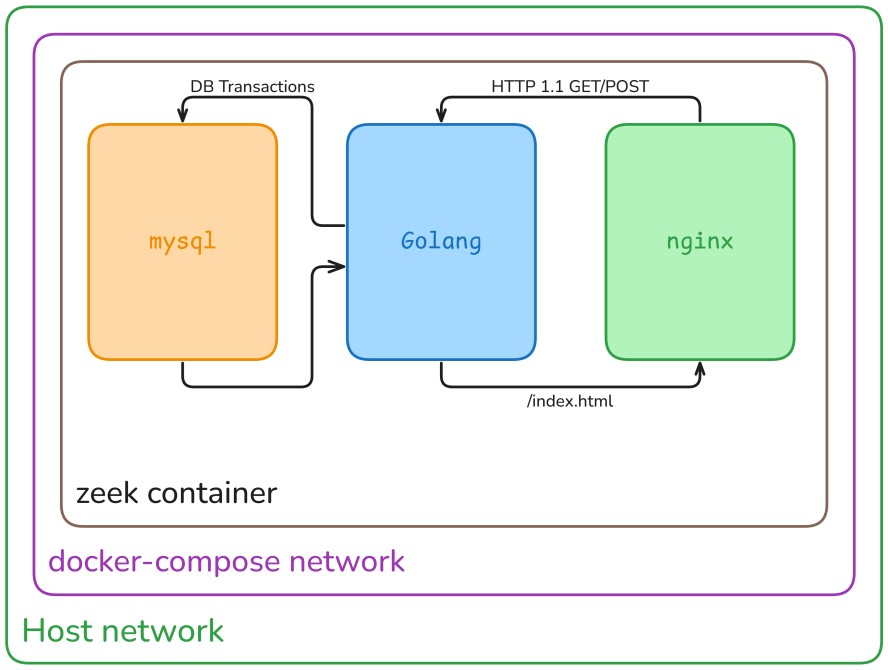
\includegraphics[width=0.7\textwidth]{image}
\caption*{\small{\textbf{Εικόνα 2.1.1} Γενική επισκόπηση της προτεινόμενης αρχιτεκτονικής}}
\end{figure}

Όλα τα παραπάνω υποσυστήματα είναι συνδεδεμένα μέσω ενός \textbf{docker-compose} αρχείου, το οποίο ρυθμίζει την επικοινωνία ανάμεσα στα containers. Το \textbf{Zeek} λειτουργεί ως το κεντρικό IDS, ενώ ο server και ο client είναι υπεύθυνοι για τη διαχείριση και την εκτέλεση αιτημάτων. Η παρακολούθηση των δικτυακών αιτημάτων και η ανταπόκριση του συστήματος γίνεται σε πραγματικό χρόνο, επιτρέπο-ντας την ανάλυση της απόδοσης των κανόνων ανίχνευσης και την αξιολόγηση της λειτουργικότητας του συστήματος.

Με αυτήν την υποδομή, καταφέραμε να δημιουργήσουμε ένα ολοκληρωμένο περιβάλλον, το οποίο είναι επεκτάσιμο και ευέλικτο, τόσο για τη δοκιμή νέων κανόνων ανίχνευσης όσο και για την προσομοί-ωση διαφορετικών σεναρίων εισβολής.


\subsection{Επιθέσεις}
Στο πλαίσιο της υλοποίησης του Intrusion Detection System (IDS) με το εργαλείο \textbf{Zeek}, δοκιμάστη-καν διάφορες τεχνικές επιθέσεων για την αξιολόγηση της αποτελεσματικότητάς του. Οι επιθέσεις χωρίζονται σε δύο κατηγορίες: χειροκίνητες επιθέσεις και αυτοματοποιημένες επιθέσεις, οι οποίες αποσκοπούν στον εντοπισμό και την ανίχνευση κακόβουλων ενεργειών από το IDS.

Αρχικά, πραγματοποιήθηκαν χειροκίνητες επιθέσεις με στόχο την εκμετάλλευση αδυναμιών σε εφαρμογές και συστήματα. Μια από τις πιο συνηθισμένες επιθέσεις ήταν το \textbf{Cross-Site Scripting} (\textbf{XSS}), το οποίο περιλαμβάνει την εισαγωγή κακόβουλου \textbf{JavaScript} κώδικα σε ιστοσελίδες, με σκοπό την εκτέλεσή του στον browser του χρήστη. Στην προκειμένη περίπτωση, χρησιμοποιήθηκε ο παρακά-τω κώδικας για να προκαλέσει την εμφάνιση του περιεχομένου του cookie του χρήστη:
\begin{lstlisting}
<img src="" onerror="alert(document.cookie);" />
\end{lstlisting}

Ένα ακόμα παράδειγμα επίθεσης ήταν η \textbf{SQL Injection}, η οποία εκμεταλλεύεται ευπάθειες στις \textbf{SQL} ερωτήσεις μιας εφαρμογής για την εκτέλεση κακόβουλων εντολών στη βάση δεδομένων. Για παράδειγμα, χρησιμοποιήθηκε η εξής εντολή:
\begin{lstlisting}
INSERT INTO Posts (title, content) VALUES ('test1', 'test2'); DROP TABLE Posts; --
\end{lstlisting}

Η επίθεση αυτή αποσκοπούσε στην εκτέλεση ενός κακόβουλου \textbf{SQL statement} για τη διαγραφή δεδομένων από τη βάση. Παράλληλα, πραγματοποιήθηκε και επίθεση \textbf{Path Traversal}, η οποία στόχευε στην πρόσβαση σε ευαίσθητα αρχεία του συστήματος μέσω κακόβουλων αιτημάτων, όπως φαίνεται στο παρακάτω παράδειγμα:
\begin{lstlisting}
curl http://localhost/api/etc/passwd
\end{lstlisting}

Αυτού του είδους οι επιθέσεις χρησιμοποιούνται για την υποκλοπή κρίσιμων συστημικών αρχείων.

Επιπλέον, εξετάστηκε η επίθεση \textbf{Buffer Overflow}, στην οποία αποστέλλονται δεδομένα μεγαλύτε-ρα του αναμενόμενου μεγέθους για να προκαλέσουν υπερχείλιση μνήμης. Η συγκεκριμένη επίθεση εκτελέστηκε με την αποστολή μεγάλου αριθμού χαρακτήρων μέσω \textbf{HTTP αιτήματος}:
\begin{lstlisting}
curl -H "Content-Type: application/json" -d '{"title":"hello world", "content":"'$
(python -c 'print("A"*5050)' | sed 's/"/\\"/g')'"}' -X POST http://localhost:1234
\end{lstlisting}

Τέλος, πραγματοποιήθηκε και μια επίθεση \textbf{Distributed Denial of Service} (\textbf{DDoS}), η οποία είχε ως στόχο τη φόρτωση του συστήματος με μεγάλο όγκο αιτημάτων, μέσω του \textbf{script ./ddos.sh}.

Από την άλλη πλευρά, χρησιμοποιήθηκαν και αυτοματοποιημένα εργαλεία για την εκτέλεση επιθέ-σεων μεγάλης κλίμακας. Ένα από τα πρώτα εργαλεία ήταν το \textbf{hping3}, το οποίο χρησιμοποιεί \textbf{TCP SYN} πακέτα για την εκτέλεση \textbf{DDoS} επιθέσεων. Ένα παράδειγμα της εντολής που χρησιμοποιήθηκε είναι η εξής:
\begin{lstlisting}
sudo hping3 -i u40 -S -p 1234 -c 1000000 172.21.0.3
\end{lstlisting}

Ένα άλλο εργαλείο που χρησιμοποιήθηκε ήταν το \textbf{Apache Bench} (\textbf{ab}), το οποίο χρησιμοποιείται για την αποστολή μεγάλου αριθμού \textbf{HTTP} αιτημάτων σε έναν server, προκειμένου να εξεταστεί η αντοχή του συστήματος υπό φορτίο. Η εντολή για την εκτέλεση της επίθεσης είναι:
\begin{lstlisting}
ab -n 100000 -c 100 http://localhost:1234/
\end{lstlisting}

Ένα ακόμα εργαλείο ήταν το \textbf{Oha}, το οποίο χρησιμοποιεί παρόμοια λογική με το \textbf{Apache Bench}, αλλά είναι σχεδιασμένο για εξαιρετικά υψηλές επιδόσεις. Η εντολή που χρησιμοποιήθηκε για την εκτέλεση του εργαλείου είναι:
\begin{lstlisting}
oha -z 2m -c 1000 http://localhost:1234
\end{lstlisting}

Τέλος, χρησιμοποιήθηκε το εργαλείο \textbf{Nmap} για την ανίχνευση ανοιχτών θυρών και την εκτίμηση της ασφάλειας του συστήματος μέσω σάρωσης υπηρεσιών και συσκευών.

Οι παραπάνω επιθέσεις καλύπτουν ένα ευρύ φάσμα κακόβουλων ενεργειών, οι οποίες αναμένεται να ανιχνευθούν και να καταγραφούν από το IDS. Συμπερασματικά, είναι φανερό ότι το \textbf{Zeek} ήταν αποτελεσματικό στην ανίχνευση των περισσότερων από αυτές τις επιθέσεις. Ωστόσο, παρατηρήθηκαν περιοχές που απαιτούν περαιτέρω βελτιώσεις, όπως η παραμετροποίηση των κανόνων για την καλύτε-ρη αναγνώριση επιθέσεων με υψηλή συχνότητα, όπως οι \textbf{DDoS} επιθέσεις.


\subsection{Κανόνες}
\subsubsection{Ανίχνευση Path Traversal}
\begin{lstlisting}
if (path_traversal_keywords in original_URI) {
    print fmt("[ALERT] Potential Path traversal detected. 
    Host: %s:%d, URI: %s", c$id$orig_h, c$id$orig_p, original_URI);
}
\end{lstlisting}
Ο πρώτος κανόνας εξετάζει αν το \textbf{URI} (Uniform Resource Identifier) που περιλαμβάνεται στο αίτημα περιέχει λέξεις-κλειδιά που σχετίζονται με τεχνικές path traversal, όπως \texttt{ ../, ..\\, /etc/passwd} ή άλλες παρόμοιες ακολουθίες. Αν ανιχνευτεί τέτοια λέξη-κλειδί, εμφανίζεται ειδοποίη-ση που περιλαμβάνει τη διεύθυνση IP του αιτούντος, την θύρα προέλευσης και το \textbf{URI} που θεωρείται ύποπτο.
\begin{lstlisting}
[ALERT] Potential Path traversal detected.
\end{lstlisting}
περιλαμβάνοντας τη διεύθυνση IP (\texttt{c\$id\$orig\_h}), την θύρα (\texttt{c\$id\$orig\_p}), και το \textbf{URI}.

Ο σκοπός αυτού του κανόνα είναι να εντοπίζει προσπάθειες παράκαμψης του προβλεπόμενου εύρους πρόσβασης σε αρχεία ή καταλόγους του διακομιστή. Αυτές οι επιθέσεις χρησιμοποιούνται συνήθως για την απόκτηση πρόσβασης σε ευαίσθητα δεδομένα ή αρχεία διαμόρφωσης που δεν θα έπρεπε να είναι προσβάσιμα από εξωτερικούς χρήστες.

\subsubsection{Ανίχνευση Code Injection}
\begin{lstlisting}
if (code_injection_keywords in full_body) {
    print fmt("[ALERT] Potential Code Injection detected. 
    Host: %s:%d, Body: %s", c$id$orig_h, c$id$orig_p, full_body);
}
\end{lstlisting}
Ο δεύτερος κανόνας ελέγχει το σώμα του αιτήματος (\textbf{full body}) για λέξεις-κλειδιά που υποδηλώνουν πιθανή \textbf{έγχυση κώδικα} (\textbf{Code Injection}), όπως \texttt{eval(), system(), ;} ή άλλες κακόβουλες εντολές. Αν τέτοια λέξη βρεθεί, εμφανίζεται ειδοποίηση που περιλαμβάνει τη διεύθυνση IP, την θύρα, και το πλήρες σώμα του αιτήματος.
\begin{lstlisting}
[ALERT] Potential Code Injection detected.
\end{lstlisting}
περιλαμβάνοντας τη διεύθυνση IP (\texttt{c\$id\$orig\_h}), την θύρα (\texttt{c\$id\$orig\_p}), και το πλήρες σώμα του αιτήματος (\texttt{full\_body}).
Ο σκοπός αυτού του κανόνα είναι η αποτροπή επιθέσεων στις οποίες οι εισβολείς προσπαθούν να εκτελέσουν αυθαίρετο κώδικα στον διακομιστή, όπως εκτέλεση \textbf{Shell Commands}, \textbf{SQL Injection}, ή άλλες παρόμοιες επιθέσεις. Η ανίχνευση τέτοιων μοτίβων μπορεί να βοηθήσει στην πρόληψη ζημιών όπως η κλοπή δεδομένων ή η αλλοίωση λειτουργιών του συστήματος.

\subsubsection{Έλεγχος μεγάλου Payload (buffer overflow)}
\begin{lstlisting}
if (|full_body| > payload_threshold) {
    print fmt("[ALERT] Payload exceeds threshold. 
    Host: %s:%d, Length: %s", c$id$orig_h, c$id$orig_p, |full_body|);
}
\end{lstlisting}
Ο τρίτος κανόνας ελέγχει το μέγεθος του σώματος του αιτήματος (payload) και το συγκρίνει με ένα \textbf{προκαθορισμένο όριο} (\textbf{payload threshold}). Αν το μέγεθος υπερβαίνει αυτό το όριο, ενεργοποιείται ειδοποίηση που περιλαμβάνει τη διεύθυνση IP, την θύρα, και το μήκος του σώματος.
\begin{lstlisting}
[ALERT] Payload exceeds threshold.
\end{lstlisting}
περιλαμβάνοντας τη διεύθυνση IP, την θύρα, και το μέγεθος του σώματος.
Ο σκοπός αυτού του κανόνα είναι να εντοπίσει περιπτώσεις όπου οι εισβολείς στέλνουν υπερβολικά μεγάλα δεδομένα σε μια προσπάθεια να προκαλέσουν ζημιά, όπως μέσω επιθέσεων \textbf{Βuffer Οverflow} ή κατάχρησης πόρων του διακομιστή.


\newpage

\section{Στιγμιότυπα Οθόνης}
\begin{figure}[H]
\centering
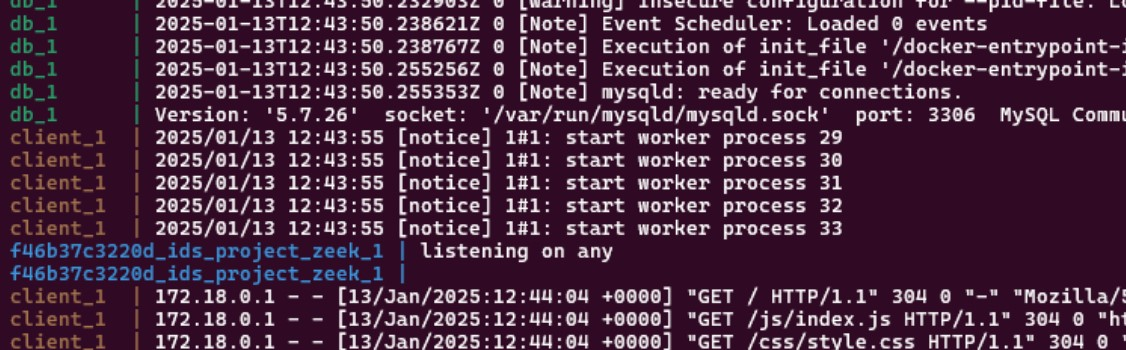
\includegraphics[width=0.8\textwidth]{containers}
\caption*{\small{\textbf{Εικόνα 3.1} Κανονική λειτουργία των \texttt{containers}}}
\end{figure}

\begin{figure}[H]
\centering
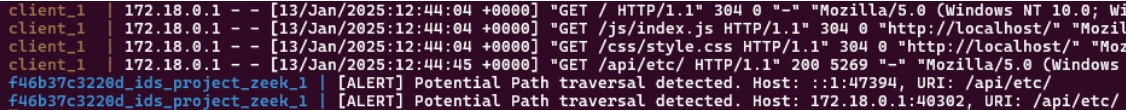
\includegraphics[width=0.8\textwidth]{potential_path}
\caption*{\small{\textbf{Εικόνα 3.2} Potential Path Traversal ALERT}}  % No extra brace here
\end{figure}

\begin{figure}[H]
\centering

\includegraphics[width=0.8\textwidth]{payload_excess}
\caption*{\small{\textbf{Εικόνα 3.3} Payload Exceeds Threshold}}
\end{figure}

\begin{figure}[H]
\centering
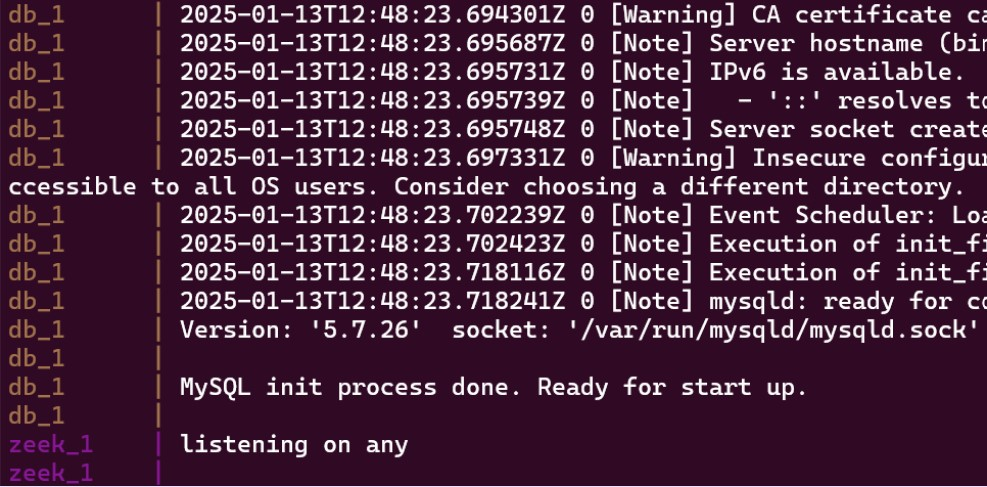
\includegraphics[width=0.8\textwidth]{listening}
\caption*{\small{\textbf{Εικόνα 3.4} Το \textbf{Zeek Container} αναμένοντας δικτυακή κίνηση}}
\end{figure}

% --- FIXED HERE (Removed one extra closing brace) ---
\begin{figure}[H]
\centering
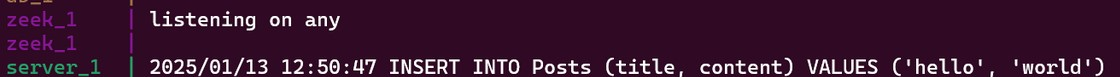
\includegraphics[width=0.8\textwidth]{curating}
\caption*{\small{\textbf{Εικόνα 3.5} Εντοπισμός νέου post από τον \textbf{Server Container}}}
\end{figure}

% --- FIXED HERE (Removed one extra closing brace) ---
\begin{figure}[H]
\centering
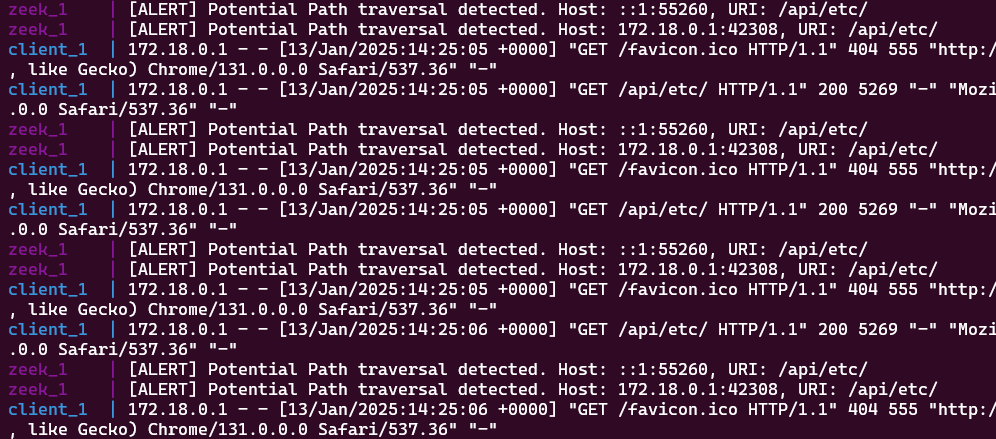
\includegraphics[width=0.8\textwidth]{alert}
\caption*{\small{\textbf{Εικόνα 3.6} Εντοπισμός πολλαπλών επιθέσεων από τον \textbf{Server Container}}}
\end{figure}

\begin{figure}[H]
\centering
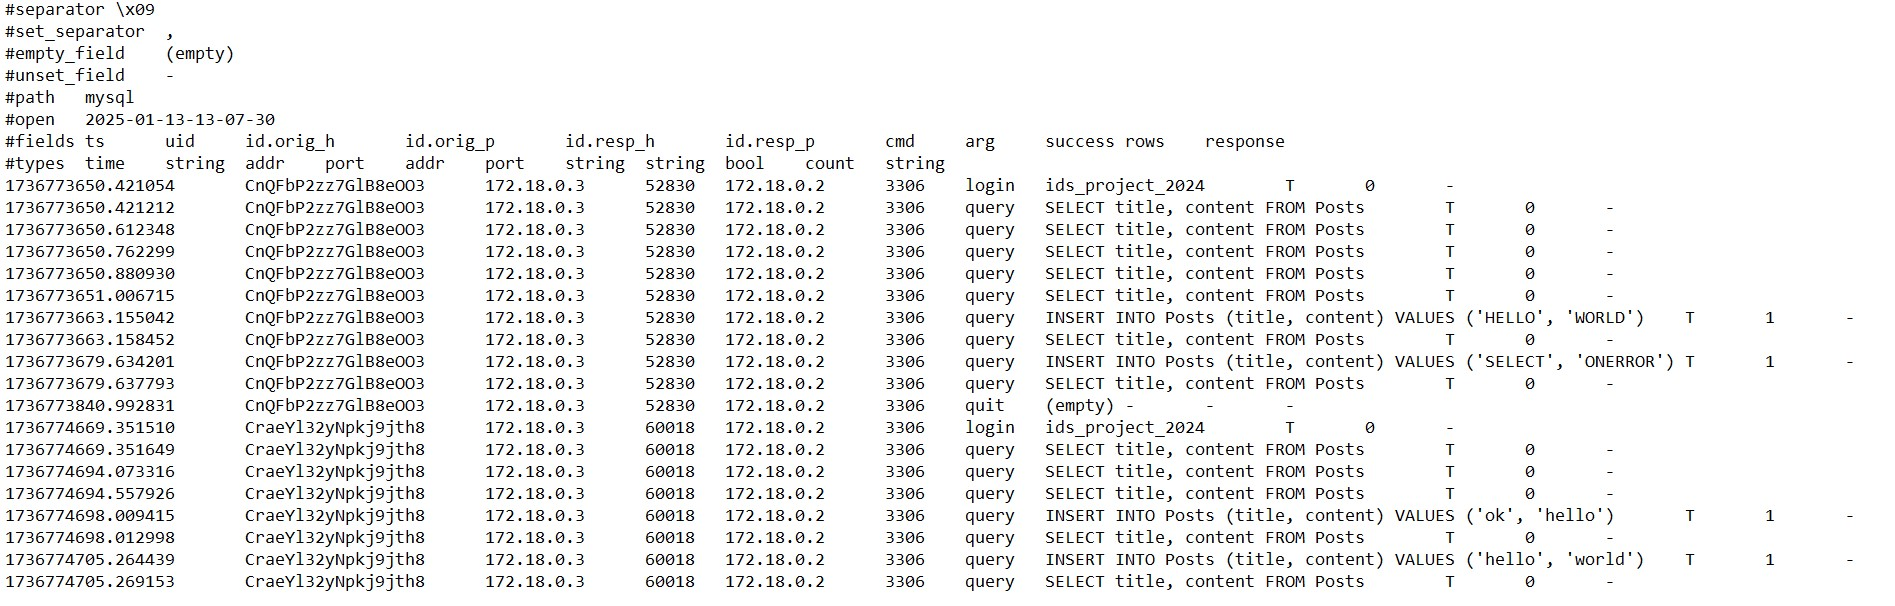
\includegraphics[width=0.8\textwidth]{mysql_log}
\caption*{\small{\textbf{Εικόνα 3.7} mysql.log}}
\end{figure}

\newpage

\section{Οπτικοποίηση}
\begin{figure}[H]
\centering
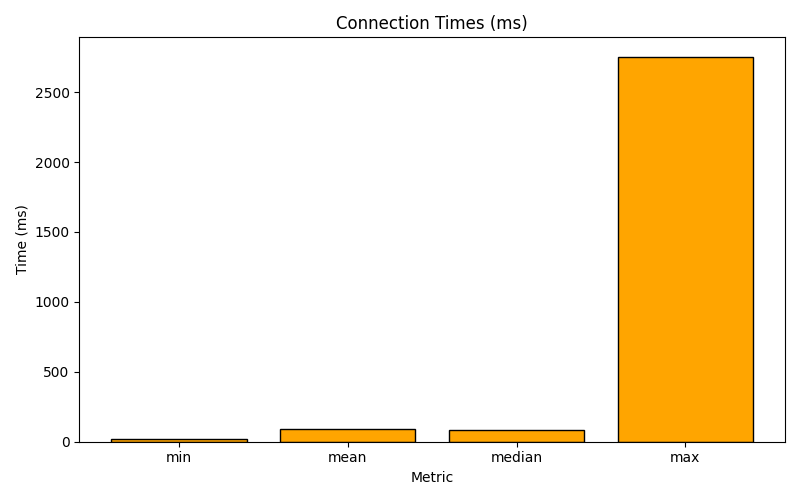
\includegraphics[width=0.85\textwidth]{ab_connection_times}
\caption*{\small{\textbf{Εικόνα 4.1} Χρονικές καθυστερήσεις συνδέσεων (ms) από με Apache Bench}}
\end{figure}

\begin{figure}[H]
\centering
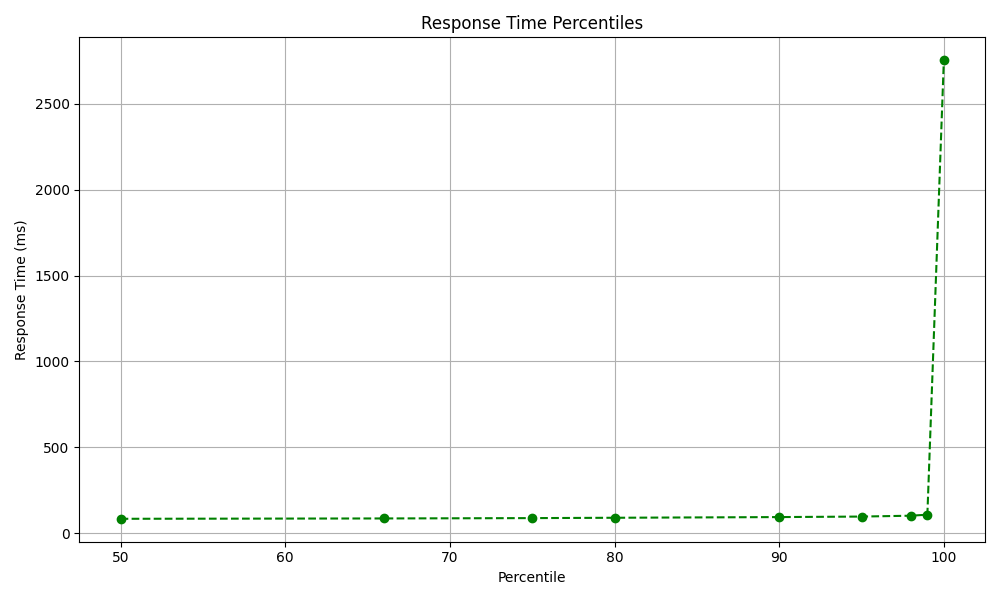
\includegraphics[width=0.85\textwidth]{ab_percentile}
\caption*{\small{\textbf{Εικόνα 4.2} Χρονικές καθυστερήσεις συνδέσεων (ms) από με Apache Bench (percentile)}}
\end{figure}

\begin{figure}[H]
\centering
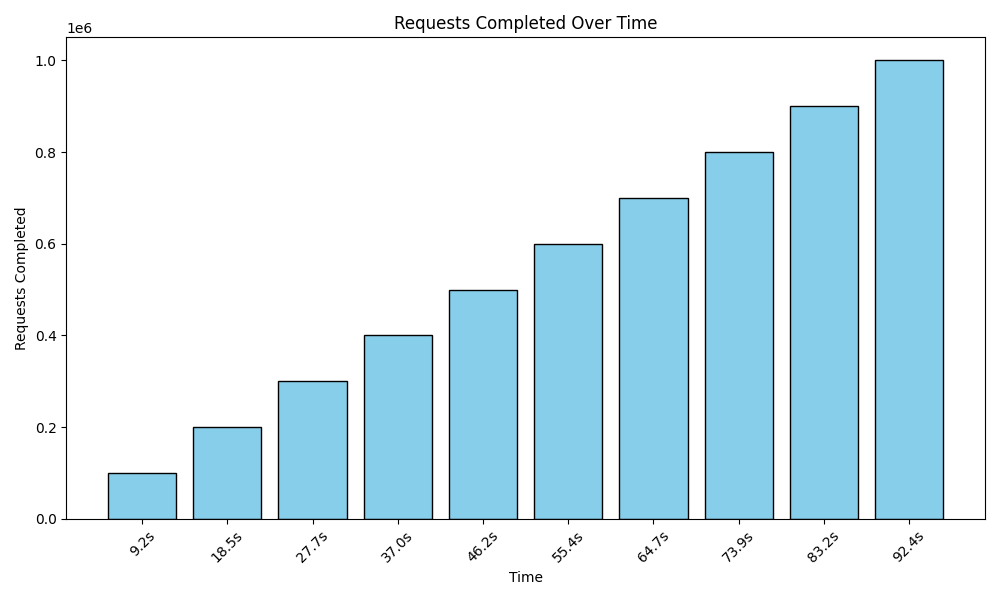
\includegraphics[width=0.85\textwidth]{ab_requests_over_time}
\caption*{\small{\textbf{Εικόνα 4.3} Ολοκληρωμένα αιτήματα με την πάροδο του χρόνου}}
\end{figure}

\begin{figure}[H]
\centering
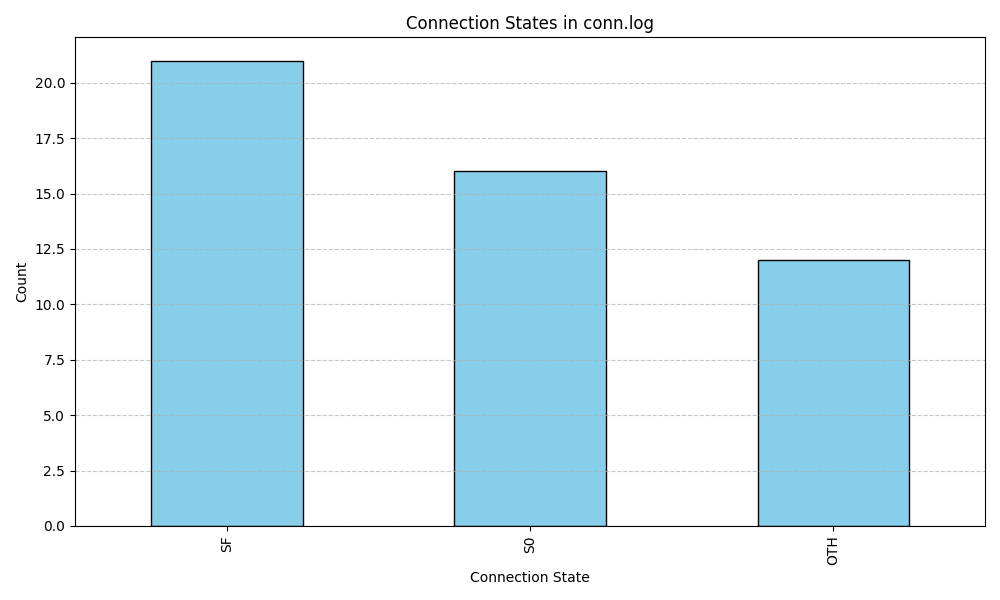
\includegraphics[width=0.85\textwidth]{connection_states}
\caption*{\small{\textbf{Εικόνα 4.4} Καταστάσεις σύνδεσης στο αρχείο conn.log: SF (Επιτυχής Σύνδεση), S0 (Προσπάθεια Σύνδεσης, Χωρίς Απάντηση), OTH (Άλλη Κατάσταση)}}
\end{figure}

Προκειμένου να οπτικοποιηθούν τα alerts που έχει παράγει το Zeek, χρησιμοποιήθηκαν τα logs που προέκυψαν. Στη συνέχεια, χρησιμοποιήθηκαν οι βιβλιοθήκες pandas και matplotlib. Επιπρόσθετα, χρησιμοποιώντας οδηγό από το \href{https://github.com/hackertarget/pcap-did-what/blob/master/zeek-docker/zeek-to-sqlite.py}{Github} μετατράπηκαν τα log files της \textbf{Zeek} σε μία \textbf{sqlite3} βάση δεδομένων όπου μετεπειτα φορτώθηκε σε ένα υπάρχον dashboard σε ένα self hosted Grafana instance.

\begin{figure}[H]
\centering
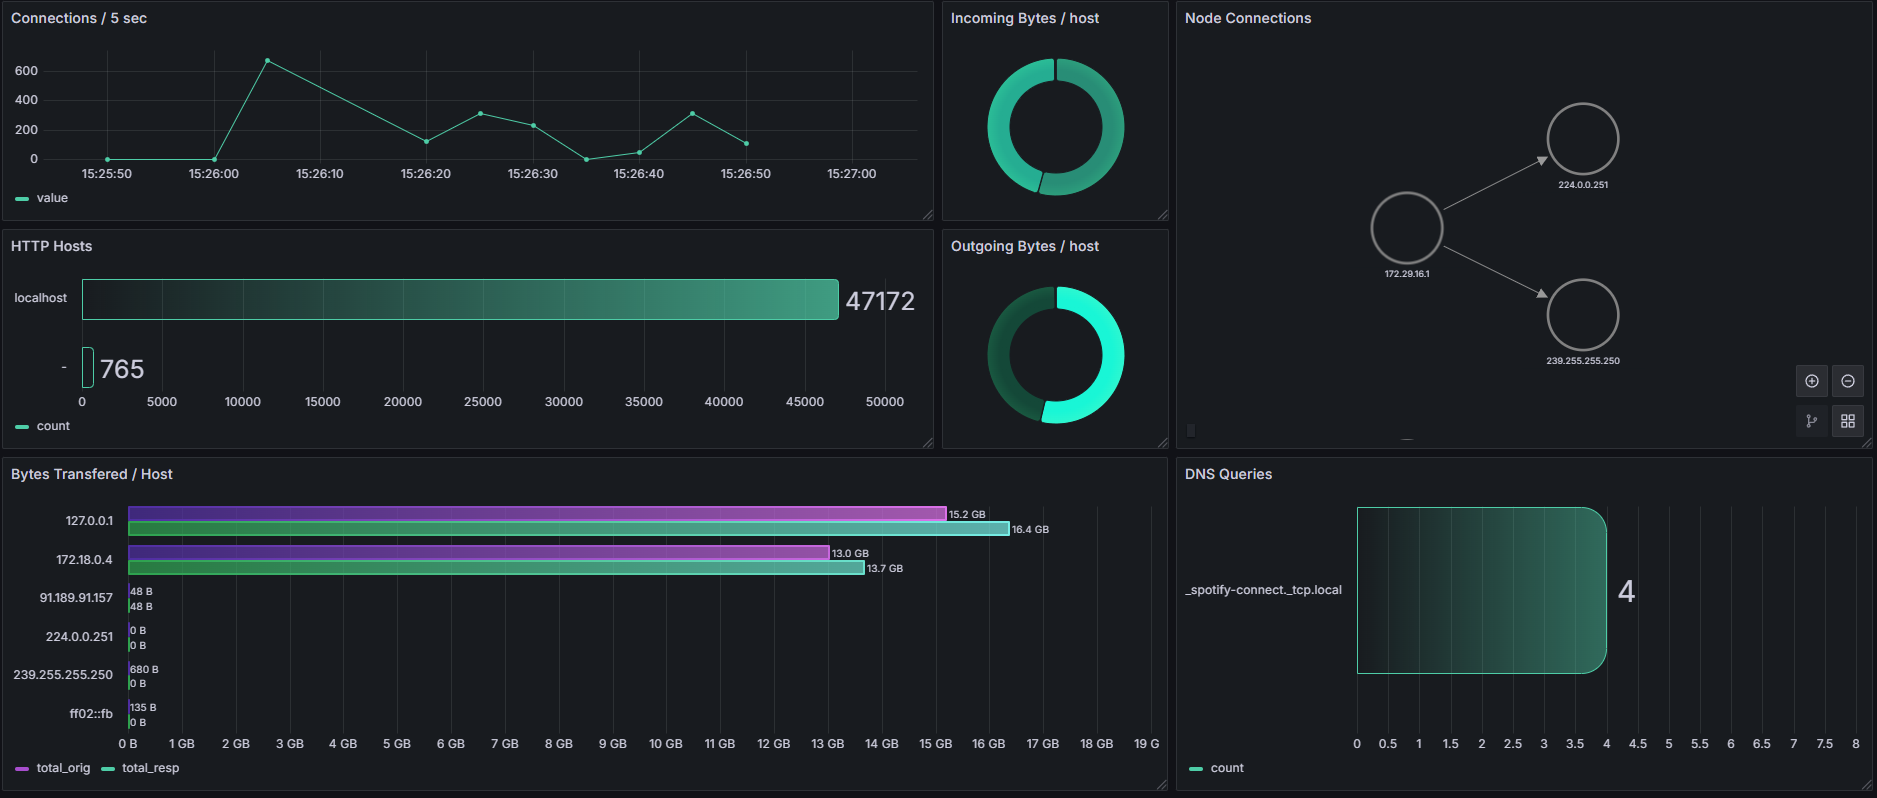
\includegraphics[width=0.85\textwidth]{graphana_og}
\caption*{\small{\textbf{Εικόνα 4.5} Το UI του \textbf{Grafana}}}
\end{figure}

\begin{figure}[H]
\centering
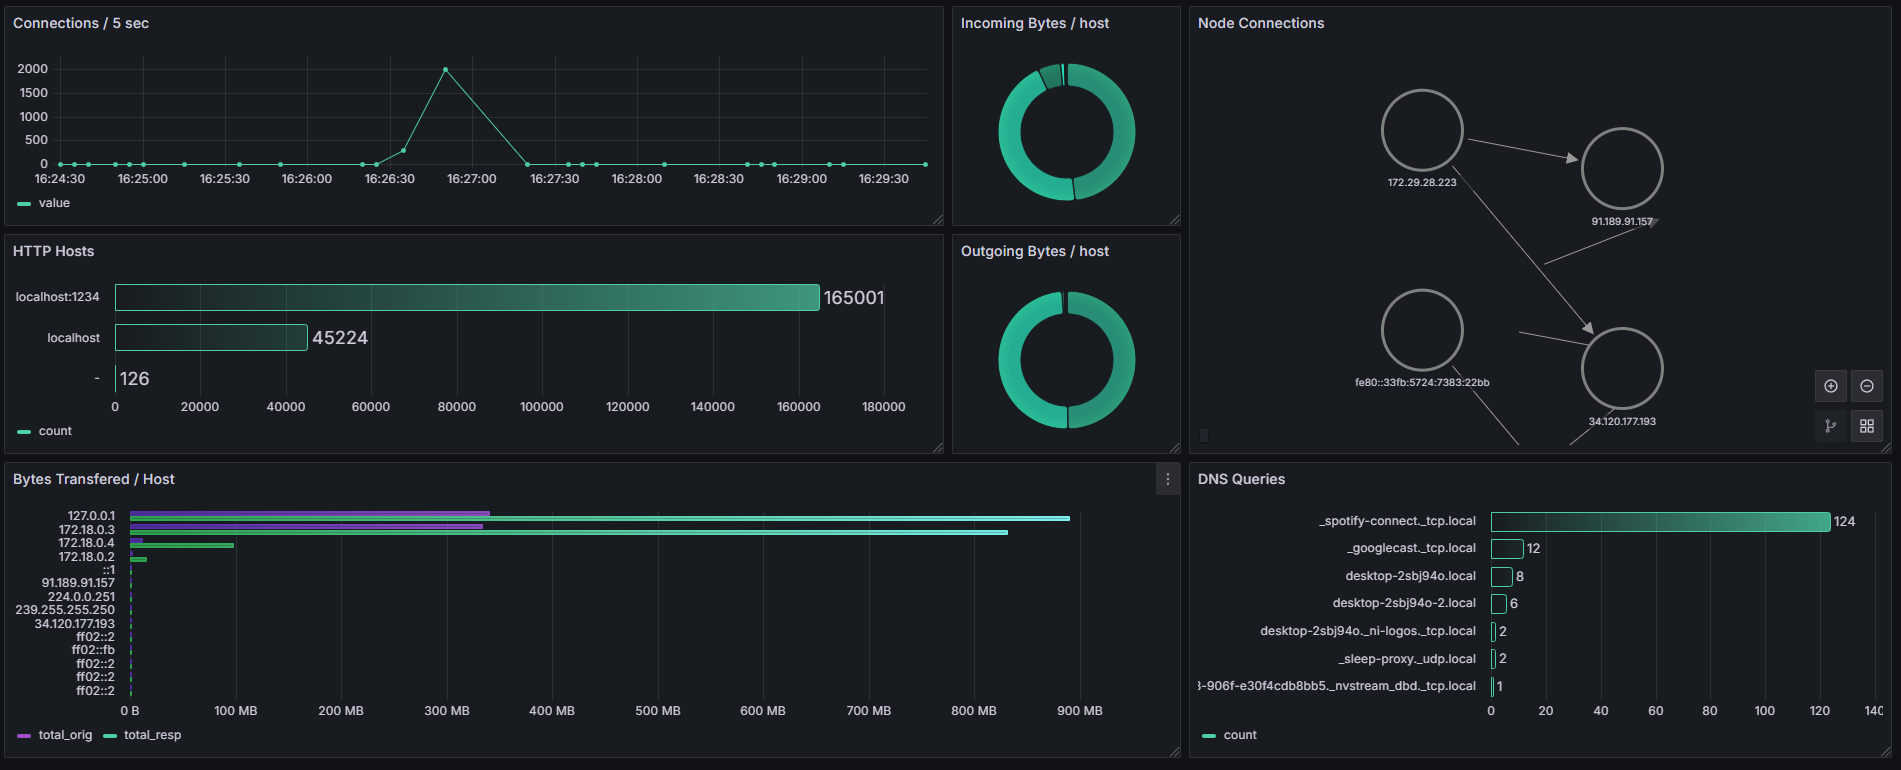
\includegraphics[width=0.85\textwidth]{graphana_1}
\caption*{\small{\textbf{Εικόνα 4.6} Το \textbf{Grafana} μετά από κάποια ώρα λειτουργίας }}
\end{figure}

\renewcommand\refname{Αναφορές}
\bibliographystyle{plain}
\bibliography{references}

\end{document}